% Versioned revision of the PR #15 review draft. Historical source/PDF unchanged.
% Venue CFP requirements verified; production template/font/PDF rebuild still pending.
\documentclass[sigconf,9pt,review]{acmart}
% Scalable preview fallback only when the ACM class reports missing fonts.
\makeatletter\if@ACM@newfonts\else\usepackage{lmodern}\fi\makeatother
\setcopyright{none}
\settopmatter{printacmref=true}
\acmConference[Review draft]{SIGMOD 2027 Demonstrations preparation}{Requirements unverified}{Not submitted}
\acmYear{2027}
\acmDOI{}
\acmISBN{}
\title{CDC Replay Correctness Lab: Making Stable but Incorrect State Visible}
% Nonanonymous track: replace the following explicit placeholder with verified author metadata before submission.
\author{Author metadata pending verification}
\affiliation{\institution{Affiliation pending verification}\country{United States}}
% Do not submit this placeholder or claim an institutional affiliation without approval.
\begin{abstract}
Change-data capture consumers can produce a stable but incorrect materialization:
identity deduplication does not order distinct changes, and finite identity memory
may hide conflicting historical payloads without changing the latest state.
CDC Replay Correctness Lab is a local, interactive demonstration of these
 distinctions. Reviewers select ordering, replay policy, checkpoint/interruption
boundaries and ID retention, inspect event-by-event decisions, and compare actual
state with an independent canonical oracle. A guaranteed stale-delete preset
reproduces baseline failure without searching seeds. Independent execution of the
original artifact reproduced its 126 principal and 36 bounded observations. New
isolated controls show that all three policies pass duplicate-only and ordered
delete/reinsert workloads; an ID-only policy still fails the stale-delete case.
A separate probe-order study exposes why retention-dependent conflict detection
cannot be inferred from final-state equality. The contribution is an inspectable,
reproducible educational/diagnostic artifact, not a new CDC algorithm or an
exactly-once guarantee.
\end{abstract}
\ccsdesc[500]{Software and its engineering~Software testing and debugging}
\ccsdesc[300]{Information systems~Data replication tools}
\keywords{change-data capture, replay, correctness oracle, interactive demonstration}
\begin{document}
\maketitle
\section{Problem and demonstration contribution}
A downstream materializer can receive a historical deletion after a newer reinsertion.
Keeping only unique event IDs does not prevent this stale overwrite when the IDs
are distinct. Moreover, a second replay may leave an already incorrect state unchanged.
A demonstration that reports only duplicate counts or redelivery stability can
therefore conceal the failure it is supposed to explain.

The lab turns these counterexamples into an audience-controlled comparison of three
simple policies. It separates \emph{final-state equality}, \emph{duplicate recognition},
\emph{conflict detection}, and \emph{recovery attempts}. A reviewer can switch from
whole-input validation to online processing and expire identities while retaining
versioned tombstones. This reveals both containment and missing detection rather
than displaying only favorable outcomes. The artifact makes established semantics
observable; it introduces no new fault-tolerance algorithm and reports no user-study
or production result.

The event contract assumes immutable identity, an authoritative comparable per-key
integer version, a string payload and a deletion flag. Higher versions determine the
intended state; tombstones remain retained. Real sources require source-specific
ordering contracts: Debezium's PostgreSQL documentation describes LSN-bearing change
events and offset-based restart~\cite{debezium}. We neither derive comparable versions
from arbitrary CDC records nor implement that connector.

\section{Architecture and correctness model}
\begin{figure}[t]
\centering
\fbox{\parbox{0.93\columnwidth}{\centering
Canonical synthetic history $\longrightarrow$ independent batch oracle\\[3pt]
$\downarrow$ scenario / ordering / failure construction\\[3pt]
Arrival $\mid$ ID-only $\mid$ version-aware processors\\[3pt]
$\downarrow$ logical checkpoint, restore, redelivery\\[3pt]
Per-event trace $+$ counters $+$ actual/oracle comparison}}
\caption{The canonical specification and replay transitions are separate. The interface
shares the tested model with the V2 experiment runner.}
\Description{Dataflow separates the canonical batch oracle from scenario generation and three replay policies, then compares their traces and final states.}
\label{fig:architecture}
\end{figure}
The system has a standard-library Python HTTP server, self-contained HTML/JavaScript,
a replay model, two research runners and artifact validators. It needs no external
service or front-end download. The installed wheel serves the same interface from
outside the checkout. Requests describe a bounded synthetic scenario; they do not
upload arbitrary client data. State is local to one request.

The independent oracle groups the canonical history by key and selects the maximum
version. Its identity and key/version ambiguity checks are separately implemented;
it calls no materializer transitions or shared processor conflict validator. It is
computed before injected delivery is processed. Hand-authored tests assert stale
updates, deletion/reinsertion and ambiguous identities/versions. This is a test
specification, not an external database authority or formal proof.

Arrival-order replay overwrites on each event. ID-only replay suppresses remembered
IDs but otherwise overwrites. Version-aware replay also refuses lower-version state
writes and conflicting equal-version values. Each principal run uses an unlimited
ID ledger. A shared preflight validator rejects conflicting input before any of the
three policies executes; that rejection must not be called online conflict detection.

At checkpoint offset $c$, logical state and ID memory are JSON-serialized. Execution
continues to interruption $i$, discards later attempts, restores the earlier snapshot
and replays from $c$. These are simulated logical checkpoints: no disk write,
fsync, transactional source/sink coupling or real crash is provided. Distributed
consistent cuts are a substantially stronger problem~\cite{snapshots}.

The trace marks pre-interruption events discarded at restore. Monotonicity counters
separate attempted writes, committed-prefix writes and recovered writes. Restore can
lower a visible version because an earlier snapshot is reinstated; it is not counted
as a stale materialization write. A completed run's correctness requires whole-state
oracle equality, independently of its redelivery stability.

\section{Live demonstration experience}
\begin{figure*}[t]
\centering
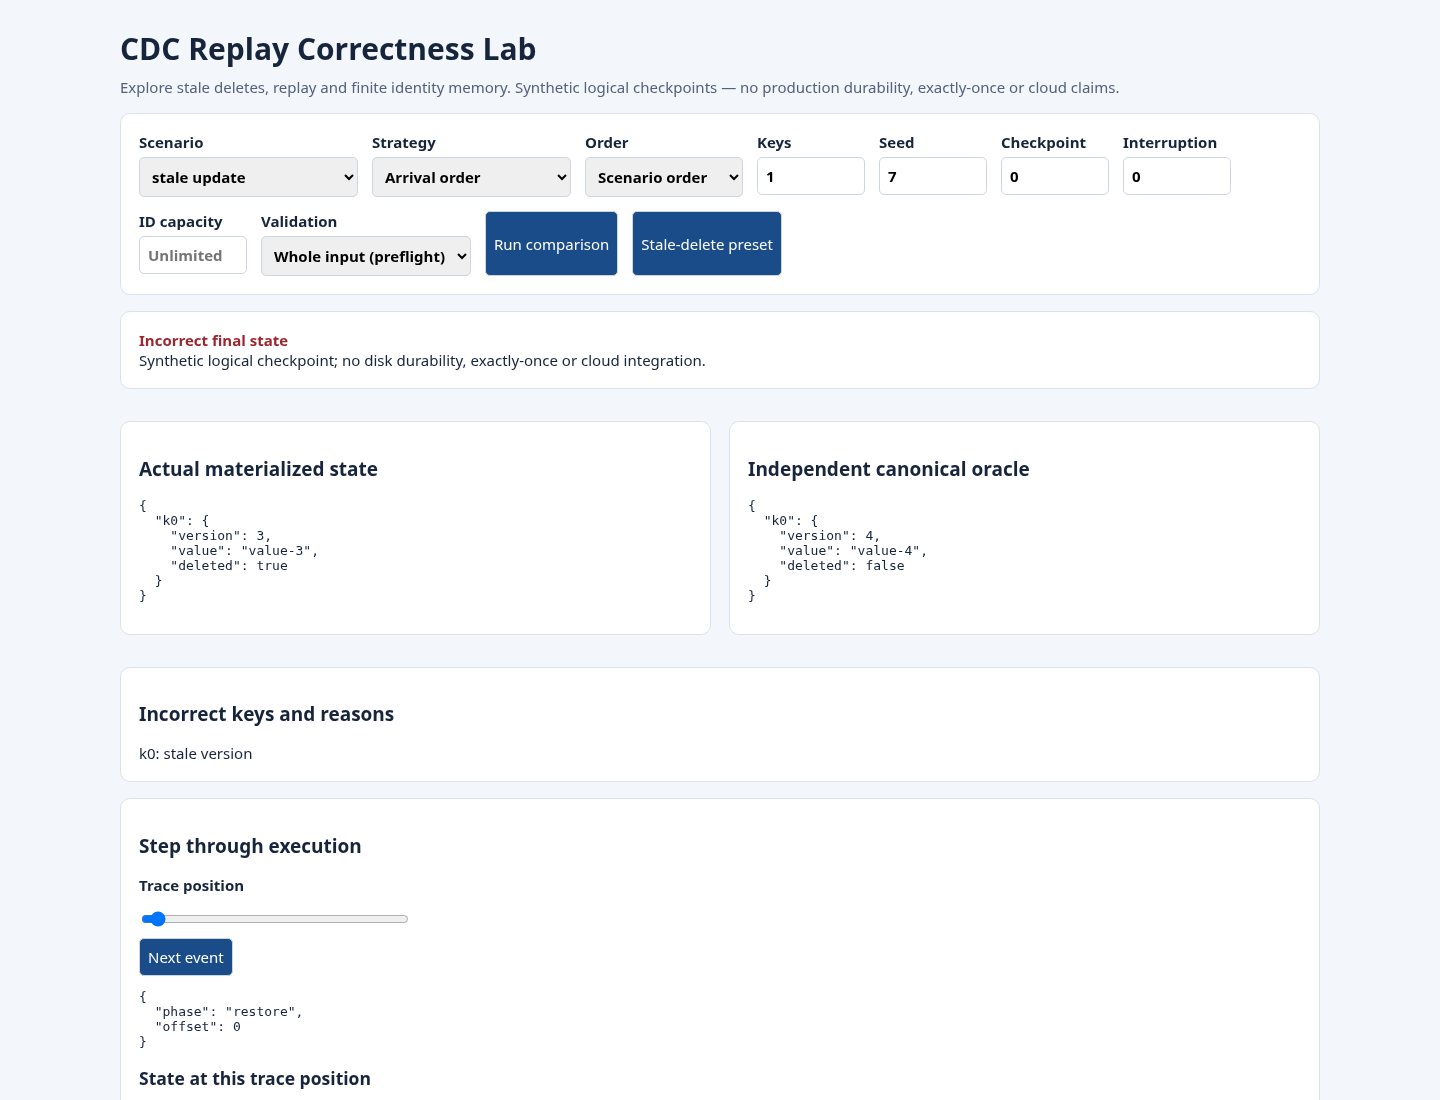
\includegraphics[width=0.88\textwidth]{figures/interactive-counterexample.png}
\caption{Actual Chromium capture of the working interface. The stale-delete preset
shows actual deleted v3 against expected live v4. Controls select strategy, ordering,
checkpoint/interruption, seed and retention; the trace slider exposes each transition.}
\Description{Browser interface showing controls, a stale-delete failure verdict, actual deleted version 3 and expected live version 4, incorrect key reason and trace controls.}
\label{fig:ui}
\end{figure*}
The interface exposes nine scenarios, policy selection, native/reversed/seeded/version
ordering, logical checkpoint and interruption offsets, and finite or unlimited ID
capacity. Side-by-side states and wrong-key explanations identify a missing key,
stale version, unexpected version, or payload/tombstone mismatch. Trace rows show
phase, source offset, event identity, applied/duplicate/stale/conflict decisions and
ledger size. A slider reveals state after the selected transition. Invalid controls
produce an explicit error; rejected or conflict-stopped runs have no completed
correctness verdict.

The five-minute walkthrough follows five interactions:
\begin{enumerate}
\item Click the stale-delete preset: one key receives live v4 under one ID and deleted
v3 under another. Arrival-order replay visibly fails within the automated one-minute
check. This case is deterministic and requires no seed search.
\item Select ID-only, then version-aware. ID-only remains wrong; version-aware keeps
live v4. Inspect the stale decision and before/after state with the trace controls.
\item Choose recovery/redelivery, three keys, checkpoint 4 and interruption 8.
Inspect four discarded attempts and four replayed lost attempts; compare final state
and the distinct redelivery-stability indicator.
\item Choose ledger expiry, 16 keys, online validation and capacity 4. Latest state
matches the oracle, yet an injected conflicting stale ID payload is not detected;
the interface explicitly warns about this distinction.
\item Clear the capacity for unlimited retention. The same conflict is detected and
processing stops. Switch to whole-input validation to see rejection before replay.
\end{enumerate}
The allocation is a presenter script, not an observed five-minute usability study.
HTTP integration tests and real Chromium automation execute the entire sequence,
including selection/filling of controls, trace stepping and absence of JavaScript
errors. The browser uses the built wheel outside the repository.

\section{Evidence and isolated controls}
The protocol was repository-committed before implementation and measurements.
A new execution of the unchanged original runner reproduced all non-timing fields
of its 126 principal and 36 bounded observations. Artifact validation checked original
and new SHA-256 manifests, CSV/JSON field parity, source/configuration hashes and
row counts. This is independent execution, not replication by a separately authored
implementation. Timing samples were intentionally not required to match.

Original duplicate and delete/reinsert conditions also shuffled input; they were
compound workloads. V2 adds truly isolated controls and records a new 144-row matrix:
8/64 keys, three seeds, eight conditions, three policies, five fresh timed executions.
Some ordered conditions do not vary with seed; rows are not independent statistical
samples. Conflicting-ID and same-version conditions yield 12 rejected inputs per
policy. The remaining 36 completed observations per policy are summarized below.

\begin{table}[t]
\caption{Completed V2 final-state outcomes; rejected inputs are excluded.}
\label{tab:results}
\centering
\begin{tabular}{lrrr}\toprule
Policy & Correct & Incorrect & Rejected\\\midrule
Arrival & 24 & 12 & 12\\
ID-only & 30 & 6 & 12\\
Version-aware & 36 & 0 & 12\\\bottomrule
\end{tabular}
\end{table}
All policies pass all six configurations each of ordered live input, duplicate-only,
ordered delete/reinsert and ordered checkpoint recovery. Thus neither duplicates
alone nor an ordered deletion/reinsertion sequence establishes an advantage for
version guards in this final-state model. Arrival and ID-only fail all six stale-delete
configurations. Reverse post-recovery redelivery additionally makes arrival replay
wrong; remembered identities contain that case for ID-only.

A separate 72-row online matrix crosses policy, capacities 0/4/16/unlimited, three
recorded seeds and two probe orders. State and tombstones remain unbounded. In
\emph{conflict-first}, version-aware replay detects the expired-ID conflict only with
unlimited memory. In \emph{exact-then-conflict}, capacities 4/16 detect it after exact
stale redelivery reinserts the ID; capacity 0 still misses it. Each configuration is
repeated over three seeds, but its ordered bootstrap is identical. A version guard
can preserve latest state while losing historical-payload consistency checks.

Five timing samples and per-row medians are retained for every observation. Timing
includes validation, snapshot copies, serialization and event traces, excluding data
construction, oracle/scoring and output I/O. Trace copying changes measured work, so
V2 timings are not used as speedups over the original runner. One host, small synthetic
streams and early rejection preclude throughput, cloud-cost or production conclusions.

\section{Related work, limits and reproducibility}
MillWheel studies persistent state and fault-tolerant streaming~\cite{millwheel}; the
Dataflow Model treats correctness/latency/cost for unordered input~\cite{dataflow}.
This lab does not reproduce either system. Its reference-specification approach sits
within established model-based testing~\cite{mbt} and reference-engine testing
literature~\cite{norec}; it does not benchmark against their techniques. Interactive
algorithm visualizations such as RaftScope~\cite{raftscope} predate this work. Our
specific demonstration joins CDC stale-delete counterexamples, attempted/recovered
trace evidence and probe-order-dependent ID expiry, rather than claiming invention
of visualization, idempotency, versions or checkpoints.

The model has no distributed scheduler, external CDC connector, durable sink,
concurrency, source epochs or tombstone garbage collection. Stable IDs and authoritative
versions are assumptions. Equal versions cannot resolve ambiguous data. Final-state
equality does not measure external side-effect multiplicity or imply exactly-once
processing. A finite ID ledger is not a bound on total state. Claims are limited to
retained deterministic workloads; independent implementation replication and a
broader prior-art review remain outstanding.

From the repository root, run \texttt{python -m unittest discover -s tests -v}, frozen
V4/V5 validation, and the V2 runner with a fresh output directory. The self-contained
interface starts with \texttt{python -m pipeline\_reliability.cdc\_interactive}.
Retained artifacts record full source commit, dirty status, Python/platform, seeds,
configurations, all samples, and workload/source/protocol hashes. Integrity checks
confirm all 85 pre-existing tracked files, including original Paper 2 artifacts, are
unchanged. Paper 1's submitted source is absent from this checkout and needs owner
overlap review; it has not been edited or imported here.

This is a versioned revision of the prior Paper 2 draft. It is \emph{not submission-ready}:
the official SIGMOD 2027 Demonstrations CFP requires a nonanonymous, 9-point ACM
\texttt{sigconf} manuscript on US Letter paper, with at most four pages including
references. The source has been adjusted to those rules, but the current PDF predates
this change and must be rebuilt. Author/affiliation metadata, current production
template/fonts, CMT submission access, and Paper 1 overlap review remain unresolved.
An optional demonstration video may be linked only once recorded and hosted. No
conference submission or automatic merge is performed.
\bibliographystyle{ACM-Reference-Format}
\bibliography{references}
\end{document}
